\documentclass[11pt, letterpaper, twoside, final]{article}
\usepackage{risk_price_inference}
\addbibresource{riskpriceinference.bib}

\author{Xu Cheng\thanks{University of Pennsylvania, \href{mailto:xucheng@upenn.edu}{xucheng@upenn.edu}}
    \and 
    Eric Renault\thanks{Brown University, \href{mailto:eric_renault@brown.edu}{eric\_renault@brown.edu}}
    \and 
    Paul Sangrey\thanks{University of Pennsylvania, \href{mailto:paul@sangrey.io}{paul@sangrey.io}}}
    
\title{Inference for the Price of Volatility Risk Under Weak Identification}

\date{\today}

\begin{document}

\begin{titlepage}


    \maketitle
    \thispagestyle{empty}
    \addtocounter{page}{-1}

    \begin{abstract} \singlespacing \noindent 
        The risk-return trade off is a central question in modern asset pricing. 
        Even though the theoretical literature cohesively argues there should be a strong positive correlation
        between expected returns and volatility, empirically measuring it has proven difficult. 
        In addition, the option pricing literature shows that volatility enters as its own risk factor, not just
        as a predictor of returns.
        Even obtaining point estimates of these risk prices in the presence of contemporaneous correlation between
        returns and volatility, the  volatility feedback effect, has proven delicate.
        We develop methods to provide  valid confidence intervals for the price of volatility and equity risk from
        equity data directly that account for this weak identification of the various parameters. 
        We do this by adapting the results in weak identification literature that uses drifting sequences in order
        to be robust to the data's identification strength. 
    \end{abstract}

\end{titlepage}

\phantomsection
\addcontentsline{toc}{section}{Introduction}

Modern finance is all about the risk return trade offs that investors face and how to optimally respond to them. 
In particular, the central question of asset pricing is what drives expected returns.
Standard economic theory predicts you must compensate investors with higher expected returns when they face more
risk.
In other words, we would expect a positive relationship between the mean and volatility of returns.
In fact, in \gentextcites{sharpe1964capital,lintner1965security} capital asset pricing model (CAPM) the expected
return varies proportionally with the volatility. 
In other words, we have a constant price of volatility risk and expected returns are perfectly correlated with
volatility.
Even in more complicated models such as the long-run risk model and rare disasters models find a very close
relationship between variance and mean of returns \parencite{bansal2014volatility, wachter2013can}.

Consequently, an important empirical question is what is the precise magnitude of this relationship.
However, unlike the consensus in the theoretical literature, the empirical literature has found pinning down this
relationship quite difficult.
Not only has its magnitude proven difficult to determine, but various estimates even differ in sign,
\parencite{lettau2010measuring}, .

The empirical literature, which we examine in more detail in the literature review, has focused on point estimates
of this magnitude. 
However, if individual investors are ambiguity averse as in \textcite{hansen2001robust, jiu2012ambiguity}, they
will care not just about how the representative investor prices volatility but also their uncertainty regarding
this estimate. 
Furthermore, when economists calibrate models, they need to know how precisely the data determine the parameters
they are calibrating.
If the need to alter the parameter value slightly in order to make their model perform well, are they bringing in
more restrictions or data to more precisely determine the parameter of interest or are they using a value that the
data tell us is incorrect?

Clearly, as obtaining precise believable point estimates of the price of volatility risk has proven quite
difficult, we should expect doing valid inference to be even more delicate.
To the best of our knowledge, this is the first paper to directly tackle this question.
Various authors report confidence intervals as well as their point estimates.
However, they do not take into account the weak identification that makes getting the point estimate difficult in
computing these estimates.

Why is it that measuring this price is so difficult when the theoretical literature is so cohesive?
Econometrically, it is because the volatility price is weakly identified, as in \textcite{andrews2012estimation},
in that the strength of the identification of the price depends upon the value of other parameters. 
This obviously begs the question --- what are these parameters? 

To estimate the risk prices, there are three different phenomena that must be distinguished.
First, the econometrician must disentangle the volatility feedback effect (leverage) which is a contemporaneous
relationship between the volatility and returns from the risk premium, which is a relationship between volatility
and expected returns. 
It is not a contemporaneous relationship, but rather a predictable one. 

Second, and just as important.
In the papers estimating the volatility expected-return relationship such as
\textcite{brandt2004relationship,lettau2010measuring} are implicitly using a one-factor model where volatility
is that factor.
However, the option pricing literature, such as  \textcite{christoffersen2013capturing}, has argued that in order
to match the option pricing data we need to include another factor.
In other there are two sources of risk that the investors face: what returns will do and what the volatility
will do.
One can view the loading on the equity risk to itself be a function of the volatility.
The econometrician can rewrite this as a two factor model with equity and volatility risk up to higher order
terms.
Since, the econometrician must disentangle these two effects, their ability to do this will depend upon various
other parameters.
As mentioned in the introduction,in CAPM we only have factor, and so clearly we cannot disentangle them.
However, most models of interest to economists nest CAPM as a special case. 
Consequently, for certain values of the parameters, the model has only one factor. 
This directly implies that we cannot separately identify the two risks for some values of the other parameters.
More generally, the identification strength of the risk prices depends upon the other parameters.
The weak identification literature shows that in these scenarios, the finite-sample distributions of the estimates
are highly nonstandard, and the usual asymptotic approximations do not perform well.


Hopefully, the reader has a high-level understanding of the issue in at hand, and why simple econometric
procedures does not provide a useful guide to the true uncertainty regarding the parameters.
The obvious next step is considering how we need to do this in practice.
Since the contribution of this paper is in terms of methodology and empirical results, we will take a model from
the literature that has the various components, instead of developing our own asset or option pricing model.
In particular, we take the model from \textcite{khrapov2016affine} and use it to estimate the relevant parameters. 

This model has a few nice features. 
First, it has both equity and volatility prices and a leverage effect. 
As such, it is the natural discrete time analogue of the \textcite{heston1993closedform} option pricing model. 
It has an exponentially affine stochastic discount factor  and shares with \textcite{heston1993closedform} the
advantage of having a structure preserving change of measure between the physical and risk-neutral models.
By doing our analysis in discrete-time we are able to more directly compare our results to risk-premia estimates
outside of the option pricing literature and the jumps in high-frequency innovations will not dramatically affect
our results.  
If we were to use a diffusion process in continuous time, we would be severely counterfactually constraining the
higher-order  moments of the process in way that would likely bias our inference. 

As far as estimation is concerned, we follow \textcite{khrapov2016affine} in using a finite version of spectral
General Method of Moments (GMM).
Effectively, we take some moments implied by the characteristic function of returns and use them in a standard GMM
setup.
The data we use are the bivariate series $\begin{pmatrix} r_{t+1}, \sigma^2_{t+1} \end{pmatrix}$.
$r_{t+1}$ is the daily return on some asset, and we use its associated realized volatility for $\sigma^2_{t+1}$.
We go into further detail in \cref{sec:data} regarding how we obtained it, the time-span covered, and so on.

\section{Literature Review}\label{sec:lit_review}


\section{The Model}\label{sec:model}

\addtocounter{subsection}{1}

We estimate the prices of some factors using moment conditions derived from an option pricing model. 
As is standard in that literature, we will do  this by specifying the physical and risk-neutral measures and their
relationship, i.e.\@ the stochastic discount factor or pricing kernel.
Let $\F_t$ be the representative investor's information set, and $P_t$ be the price on the asset in question, with
associated return $r_{t+1}$ and volatility  $\sigma^2_{t+1}$.

Given $\F_{t}$, the vector $\left( r_{t+1},  \sigma^2_{t+1}\right)$ is drawn from some process --- $\PP$ --- the
physical measure. 
We can further define the risk neutral measure --- $\QQ$ ---  as the process that makes $P_t$ a martingale, i.e.\@
the following holds. 
The advantage of defining $\QQ$ is that for some payoff function --- $f$  -- that is a function of future return
--- $r_{t+1}$ and volatility $\sigma^{t+1}$ and potentially depends upon the current information available --
$\F_t$, we can price this payoff as its expectation with respect to $\QQ$.
In other  words, the price of $f(r_{t+1}, \sigma^2_{t+1}, \F_t)$ satisfies for all $t$ and for all $f$.
This is useful because we can choose $f$ as a convenient function for our estimation. 

\begin{equation}
    P_t(f) = \E_{\QQ}\left[ f\left(r_{t+1}, \sigma^2_{t+1}, \F_{t}\right)  \mvert \F_{t}\right]
\end{equation}

Since $P_t(f), r_{t+1}$ and $\sigma_t^2$ are observable, if we specify a model for $\F_t$ in terms of observable
(to the econometrician) variables, this provides a moment condition that we can use. 
However, this condition does not identify everything we wish to estimate, in particular it does not identify the
risk prices. 


To see this, we complete the model by defining the stochastic discount factor --- $M_{t, t+1}$ --- as the
Radon-Nikodym derivative between the $\PP$ and $\QQ$ measures. 
No arbitrage guarantees that this will exist, \parencite{harrison1978martingales}.
Since risk prices arise from investors' demand for compensation to hold risk, i.e.\@ their risk-aversion, here is
where they show up in the $\QQ$ measure. 
(We collect the parameter of interest into a vector --- $\eta$.)


\begin{defn}{Asset Pricing Moments}
    \begin{equation}
        P_t(f)  = \E_{\QQ} \left[f\left(r_{t+1}, \sigma^2_{t+1} , \F_t\right) \mvert \F_t \right] =
        \E_{\PP}\left[M_{t,t+1}(\eta)f\left(r_{t+1}, \sigma^2_{t+1}, \F_t\right) \mvert \F_t \right] 
    \end{equation}
\end{defn}

\subsection{Dynamics}

To specify the model we must specify what the $\PP$ and $\QQ$ measures are and what $M_{t, t+1}(\eta)$ is.
We start by specifying the $\PP$ measure.

Following \textcite{khrapov2016affine}, we specify the joint dynamics of $\left(r_{t+1}, \sigma^2_{t+1}\right)$
under $\PP$ using Compound Autoregressive models (Car) of \textcite{darolles2006structural}.
These models are autoregressive models for the Laplace transform of the process.
The leading parameterization is the autoregressive gamma process (ARG) of \textcite{gourieroux2006autoregressive}.

In particular, we assume that the variables are first-order Markov and there is no Granger causality from return
to the volatility and that returns are serially independent given the volatility path.
In other words, the volatility drives all of the dynamics of the process.
Note, we do allow $\sigma^2_{t+1}$ and $r_{t+1}$ to be contemporaneously correlated.
They are in the data.

Since the Laplace transform is an expectation of a specific function, by assuming the data are jointly CAR(1), we
can represent out model under the physical  as follows for some functions $a_{\PP}, b_{\PP}, \alpha_{\PP},
    \beta_{\PP}$, and $\gamma_{\PP}$ for all $u$ in its domain.

\begin{defn}{The Model under the Physical Measure}
    \label{defn:physical_model}
    \begin{align}
        \E_{\PP} \left[\exp(-u \sigma^2_{t+1}) \mvert \sigma^2_t\right] &= \exp\left( - a_{\PP}(u)
            \sigma^2_{t} - b_{\PP}(u) \right) \\
        \E\left[\exp(-u r_{t+1}) \mvert \sigma^2_{t},  \sigma^2_{t+1}\right] &= \exp\left(- \alpha_{\PP}(u)
        \sigma^2_{t+1} - \beta_{\PP}(u)\sigma^2_{t} - \gamma_{\PP}(u) \right) 
    \end{align}
\end{defn}

The model in \cref{defn:physical_model} is parameterized using the functions mentioned and at this level of
generality fully nonparametric. 
To gain tractability, we will specify these function below obtaining a parametric model.
In other words, we replace the infinite degrees of freedom in \cref{defn:physical_model} with a parameter vector
with finite degrees of freedom.

First, we assume that the volatility follows an autoregressive gamma process---ARG(1), and so its physical measure
dynamics are governed by following equations.

\begin{gather}
    a_{\PP}(x) = \frac{\rho x}{1 + c x}  \\
    b_{\PP}(x) = \delta \log \left(1 + c x\right) \\
    \rho \in [0, 1), c > 0, \delta > 0 
\end{gather}

In order to interpret these parameters, it is useful to note the formula for the conditional mean
\parencite[8]{khrapov2016affine}.
As we can see, $\rho$ is a persistence parameter, and $\delta$ is a drift.
The parameter $c$ scales the volatility.

\begin{equation}
    \E\left[\sigma^2_{t+1} \mvert \sigma^2_t\right] = c \delta + \rho \sigma^2_t
\end{equation}

Before, we discuss how we parameterize the Laplace function for the return process, we will consider the $\QQ$
measure.
We will assume that the risk-neutral measure is structure preserving.
In other words, the Laplace functions maintain the same structure for some functions some functions $a_{\QQ},
b_{\QQ}, \alpha_{\QQ}, \beta_{\QQ}$, and $\gamma_{\QQ}$.
This is a relatively weak assumption because the absolute continuity of the two measures places strong
restrictions on deviations from this case.
For example, in the continuous-time limit this structure-preserving relationship would always hold.


\begin{defn}{The Model under the Risk-Neutral Measure}
    \label{defn:risk_neutral_model}
    \begin{align}
        \E_{\QQ} \left[\exp(-u \sigma^2_{t+1}) \mvert \sigma^2_t\right] &= \exp\left( - a_{\QQ}(u)
            \sigma^2_{t} - b_{\QQ}(u) \right) \\
        \E\left[\exp(-u r_{t+1}) \mvert \sigma^2_{t},  \sigma^2_{t+1}\right] &= \exp\left(- \alpha_{\QQ}(u)
        \sigma^2_{t+1} - \beta_{\QQ}(u)\sigma^2_{t} - \gamma_{\QQ}(u) \right) 
    \end{align}
\end{defn}

Since the Laplace transform for $r_{t+1}$  is exponentially affine under both $\PP$ and $\QQ$, the measure change
between them is also exponentially affine.
If we let $\pi$ be the price of volatility risk and $\theta$ be the price of equity risk, we can write down the
change of measure as follows.
We let $r_{f,t}$ be the risk-free rate.
It deterministically discounts the prices but plays no further role in the analysis.


\begin{defn}{The Stochastic Discount Factor}
    \begin{equation}
        M_{t,t+1}(\pi, \theta) = \exp\left(-r_{f,t}\right) \exp\left(m_{0}(\pi, \theta) + m_1(\pi, \theta)
        \sigma_t^2 - \pi \sigma^2_{t+1} - \theta r_{t+1}\right) 
    \end{equation}
\end{defn}

\purple{The next thing to do is to show how we replace the unspecified functions and convert them to some moments
that we can use.}

\begin{gather}
    \intertext{Then by the law of iterated expectations and some algebra.}
    \E \left[\exp\left(m_{0}(\theta) + m_1(\theta) \sigma_t^2 - \pi \sigma^2_{t+1} - \theta r_{t+1}\right)
    \exp\left(- \alpha(\theta) \sigma^2_{t+1} - \phi (\theta) \sigma^2_{t+1} - \gamma(\theta)\right) \mvert
    \F_t \right] = 1
\end{gather}

To estimate this equation, we need to know all of the relevant functions.
The parametric structure of the problem and some algebra implies the following.

\begin{align}
    a(x) &= \frac{\rho x}{1 + c x} \\
    b(x) &= \delta \log \left(1 + c x\right) \\
    \alpha(x) &= \psi x - \frac{1}{2} x^2 (1 - \phi^2) \\
    \label{eqn:beta_defn}
    \beta(x)  &= x \alpha_{\QQ}\left(- \frac{\phi}{\sqrt{c [1 + \rho]}} \right) \\
    \label{eqn:gamma_defn}
    \gamma(x) &= x b_{\QQ}\left(- \frac{\phi}{\sqrt{c [1 + \rho]}}\right) 
\end{align}

In last two of the above equations we have the risk-neutral $\alpha_{\QQ}(x)$ and $\beta_{\QQ}(x)$ functions which
we have not defined.
To solve for them we drive the implied stochastic discount factor and make the appropriate measure change.
We parameterize the SDF in terms of price of volatility risk---$\pi$---and the price of equity
risk---$\theta$.  
The SDF satisfies the following equation for some functions $m_0(\cdot)$ and $m_1(\cdot)$.


This implies the two unspecified functions are as follows.

\begin{align}
    m_{0}(\theta) &= \gamma(\theta) + b\left(\alpha\left(\theta\right) + \pi\right) \\
    m_{1}(\theta) &= \phi(\theta) + a\left(\alpha(\theta) + \pi\right) 
    \intertext{Now we can solve for $\alpha_{\QQ}(x)$ and $\beta_{\QQ}(x)$.}
    a_{\QQ}(x) &= a\left(x + \pi + \alpha(\theta)\right) - a\left(\pi + \alpha(\theta)\right) \\
    b_{\QQ}(x) &= b\left(x + \pi + \alpha(\theta)\right) - b\left(\pi + \alpha(\theta)\right) 
\end{align}

We substitute them back into \cref{eqn:beta_defn} and \cref{eqn:gamma_defn} eliminating $\alpha_{\QQ}(x)$ and
$\beta_{\QQ}(x)$.

\begin{align}
    a(x) &= \frac{\rho x}{1 + c x} \\ \label{eqn:a(x)}
    b(x) &= \delta \log \left(1 + c x\right) \\ \label{eqn:b(x)}
    \alpha(x) &= x \left(\frac{\phi}{\sqrt{c (1 + \phi)}}  + (1 - \phi^2)\left(\theta - \frac{1}{2}\right)\right)
    - \frac{1}{2} x^2 (1 - \phi^2) \\ \label{eqn:alpha(x)}
    \beta(x)  &= x \left(a\left(-\frac{\phi}{\sqrt{c(1+ \rho)}} + \pi + \alpha(\theta)\right) -
        a\left(\pi + \alpha(\theta)\right)\right) \\ 
        \label{eqn:beta(x)}
    \gamma(x) &= x \left(b\left(-\frac{\phi}{\sqrt{c(1+\rho)}} + \pi + \alpha(\theta)\right) -
        b\left(\pi + \alpha(\theta)\right) \right)
\end{align}


The set of parameters we want to estimate is $\eta \coloneqq \lbrace c, \rho, \delta, \phi, \pi,
\theta\rbrace$.

\section{Finite Spectral GMM}
\label{sec:spectral_GMM}

We derive a set of moment conditions from the characteristic function above by evaluating it at a grid of points
in $[0,1] \times i [0,1]$. 
That is we can define a function $g_t(x, \eta)$

\begin{defn}{Moment Conditions}
    \begin{equation}
        g_t(x, \eta) \coloneqq Z_t \otimes \begin{bmatrix} \exp(- x \sigma^2_{t+1}) - \exp\left( - a(x) \sigma_t^2
        - b(x) \right) \\ \exp\left(- x r_{t+1}\right) - \exp\left(- \alpha(x) \sigma^2_{t+1} - \beta(x)
        \sigma^2_t - \gamma(x)\right) \end{bmatrix}
    \end{equation}
\end{defn}

Where the instruments are given by \cref{defn:instruments} for complex unit $i$. 

\begin{defn}{Instruments}
    \label{defn:instruments}
    \begin{equation}
        Z_t = \left[1, \exp\left(- i \sigma_{t-1}^2\right), \exp\left(-i \sigma^2_{t-2}\right)\right] 
    \end{equation}
\end{defn}

The implied unconditional moment restrictions are the following.  

\begin{equation}
    \E \begin{bmatrix}  \mathrm{Re} (g_t(x, \eta)) \\ \mathrm{Im} (g_t(x, \eta)) \end{bmatrix} = 0
\end{equation}


The optimal weighting matrix has its standard form as the precision matrix of the moments as long as we choose a
finite gird for $x$. 
If we use the entire continuum, handling the weights becomes more delicate. 
So we use only finitely many moments for now.


\begin{restatable}[Identified Set]{lemma}{identifiedSet}
    \label{lemma:IdentifiedSet}
    Let $\eta_0 \coloneqq \left(\rho_0, c_0, \phi_0, \pi_0, \theta_0\right)$.
    Let the domain $\Eta$ for $\eta$ be defined as follows. 
    \begin{equation}
    \begin{split}
        \Eta &\coloneqq \left\{ \eta \in  [0, \overline{\rho}] \otimes [0, \overline{c}] \otimes \left[-1,
            1\right] \otimes \left[-\underline{\theta}_1, \overline{\theta}_1\right] \otimes
            \left[-\underline{\theta}_2, \overline{\theta}_2\right]\right\} \\
        &0 < \overline{c}, -\underline{\theta}_1, \overline{\theta}_1, -\underline{\theta}_2 < \infty, 0 <
            \overline{\rho} < 1
    \end{split}
    \end{equation}


    \begin{equation}
        \text{Given}\ \eta_0 \in \Eta,\ \text{the moment conditions}\ g_t(x, \eta)\ \text{identify}\
    \begin{cases}
        \eta_0                  &\text{if}\ \phi \neq 0 \\
        \eta_0 \setminus \pi_0  &\text{if}\ \phi = 0
    \end{cases}
    \label{eqn:EtaDefn}
    \end{equation}

    In addition, if $\phi = 0$, the GMM criterion function is independent of $\theta$.
\end{restatable}


If we plug in the estimated values of the parameters from \textcite{khrapov2016affine} into $\frac{\partial
\phi}{\partial \pi}$ and plot it as a function of $\phi$,  we get the following.
The scale is omitted because it is not meaningful. 
As can clearly be seen in \cref{fig:fig:gamma_diff_theta2}, there is a zero when $\phi = 0$.

\begin{figure}[htb]
    \centering
    \caption{Derivative of $\gamma(x)$ with respect to $\theta$}
    \label{fig:fig:gamma_diff_theta2}
    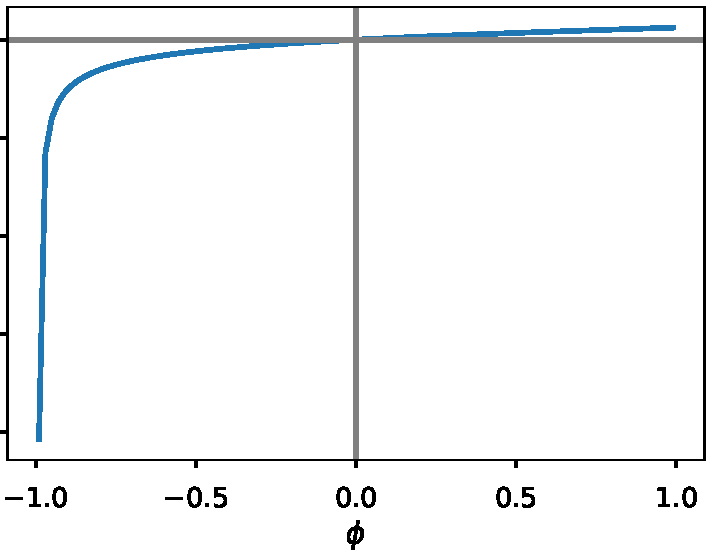
\includegraphics[width=.5\textwidth]{gamma_diff_theta2.pdf}
\end{figure}

\begin{restatable}[Uniform Convergence under Strong Identification]{lemma}{UllnStrongID}
    \label{lemma:UniformConvergenceStrongID}
    Let $\Eta$ be the identified set defined by \cref{eqn:EtaDefn}.
    Further assume that $\phi_0 \neq 0$. 
    Let $\sampmom$ be the sample moment condition defined above, and $\W_T$ be the associated optimal weight matrix
    estimator.
    Then we have the following convergence.

    \begin{align}
        &\sup_{\eta \in \Eta} \norm*{\sampmom(\eta) - \E\left[g\left(\eta \mvert \gamma_0\right)\right]}_{Fro}
          \pto 0 \\ 
        &\sup_{\eta \in \Eta} \norm{\W_{T}(\eta)-\E\left[\W\left(\eta \mvert \gamma_0\right)\right]} \pto 
    \end{align}

\end{restatable}



%TODO where does this go?
By the above arguments, we have a consistent estimator for $\eta$ and the optimal weight matrix $\W \coloneqq
(\E\left[g g'\right])^{-1}$, and we will assume that the true value $\eta_{0}$ is in the interior of its sample
space $\Eta$.\footnote{Throughout we will use subscript \num{0}  to denote true values for parameters.}
Let $G \coloneqq \E\left[\frac{\partial}{\partial \eta} \popmom \right]$
Clearly, $g$ is continuously differentiable, and its derivative $G$ is continuous.
In addition, by the identification discussion $G' W \nabla G$ is nonsingular.

%TODO Replace this with strong (alpha) mixing of order (1+\epsilon). 
%Don't you need a lot more than this...?

\begin{assump}[Weak Dependence]
    \label{assumption:weak_dependence}
    $z_t \coloneqq \begin{pmatrix} r_{t+1} \\ \sigma^2_{t+1} \end{pmatrix}$ are $\alpha$-mixing with $\alpha_t =
       O\left(T^{-5}\right)$
\end{assump}

Since, $\norm*{g_t}$ is almost surely bounded by $1$ it has all of its moments and $z_t$ being $\alpha$-mixing
implies $g_t$ is as well by the central limit theorem for strongly mixing process 
$\sqrt{T} \sampmom(\eta^{*}) \dto \N\left(0, \E\left[\W\right]^{-1}\right)$ as required. 
Consequently, by \textcite[theorem 3.2]{newey1994large} we have convergence in distribution as well as convergence
in probability.

\begin{theorem}[Inference for $\eta$ under Strong Identification]
    Assume that $\phi_0  \in (-1,1) \setminus 0$, $\rho_0 \in [0,1)$, and $c_0 > 0$. 
    Further assume that the data are ergodic, stationary, and satisfy \cref{assumption:weak_dependence}.
    Then the following convergence in distribution holds.

    \begin{equation}
    \sqrt{T} (\widehat{\eta}_T - \eta_0) \dto \N\left(0, \left(G' \E[\W] G\right)^{-1}\right)
    \end{equation}
\end{theorem}





\section{Weak Identification Setup}

In this section, take the model described in the previous sections and place it in the setup of
\textcite{andrews2014Gmm} so that we ca analyze the effects of possible lack of identification in the model in a
nice clean way.
The goal here is to perform valid inference for $\pi, \theta$ even when $\phi$ might be zero. 


From the discussion above, we can collect the parameters discussed above into a parameter vector of the following
form,i.e.\@ recall the following: $\eta = \lbrace \rho, c, \delta, \phi, \pi, \theta \rbrace$
To write it in the notation of \textcite{andrews2014Gmm}, we partition $\eta$ into three subsets.

\begin{align}
    \phi &\coloneqq \phi  \in (-1, 1) \\ 
    \zeta &\coloneqq \lbrace \rho, c, \delta, \theta \rbrace \in [0,1) \times \R_{++} \times \R_{++} \times
    \R  \\
    \pi &\coloneqq \pi \in \R 
\end{align}

Let $\Eta$ be the set of possible $\eta$, that as defined above.
It is worth noting that the parameter space has a product form, i.e.\@ the values do not affect the valid values
of the other parameters.

In this environment, $\pi$ is not identified when $\phi = 0$.
Both $\phi$ and $\zeta$ are always identified, and $\zeta$ does not affect the identification of $\pi$.

Let $Q_T(\eta)$ be the GMM criterion function, then the GMM estimator $\hat{\eta}_T$ satisfies the following.


\begin{equation}
    \widehat{\eta}_T \in \Eta\ \text{and}\ Q_T(\hat{\eta}_T) = \inf_{\eta \in \Eta} Q_T(\eta) +
    o\left(T^{-1}\right) 
\end{equation}


Now that we have defined the parameters, we can characterize the set of assumptions necessary for valid inference.
We will work through the assumptions described in \textcite{andrews2014Gmm}.
The set of necessary assumptions is relatively complicated because we have to characterize the asymptotic
distribution under several different estimation strengths simultaneously, and the assumptions required to do that
  differ in the various cases. 
In what follows, we will use 

The first assumption specifies the basic identification
problem. It also provides conditions that are used to determine the
probability limit of the GMM estimator, when it exists, under all categories
of drifting sequences of distributions.
Let $\xi$ index the part of the distribution of the data $r_{t+1}, \sigma^2_{t+1}$ that is not determined by the
moment equations.
In general, it is a (likely infinite-dimensional) nuisance parameter that affects the distribution of the data. 


We collect the parameters that we are estimating $\eta$ and the nuisance parameter $\xi$ into one parameter,
$\gamma$ and associated parameter space $\Gamma$.
In the previous discussion we characterized the parameter spaces in a non-compact fashion, let $\Eta^{*}$ be a
compact subset of $\Eta$, where the true parameter values live.
%TODO Does the set of possible nuisance parameters depend upon the estimated parameters in our model?

\begin{defn}{Complete Parameter Space}
    \begin{equation}
        \Gamma \coloneqq \left\lbrace \gamma = (\eta, \xi) \mvert \eta \in \Eta, \xi \in \Xi \right\rbrace 
    \end{equation}
\end{defn}

We characterize these drifting sequences of distributions by sequences of true parameters $\gamma_T \coloneqq
(\eta_T, \phi_T)$.

\purple{TODO Add discussion of the limiting process.}
\purple{Verify that the assumptions on the parameter space hold.}
\purple{Discuss what happens if we lack identification and hence cannot consistently estimate the parameter.}

\begin{restatable}[Inference for $\eta$ under Weak Identification]{theorem}{InferenceWeakID}
    Let that $\phi_0  \in (\underline{\phi}_0,1)$, for some $\underline{\phi}_0 > -1$. 
    $\rho_0 \in [0,1)$, and $c_0 > 0$. 

    \purple{TODO  Add Conclusion}
\end{restatable}


\section{Simulations}

\section{Data}\label{sec:data}

We also assume that $\left[ \frac{\psi}{\phi} \right]^2 \approx \frac{\E \left[\sigma^2_{t+1} \mvert
\F_t\right]}{\Var\left[r_{t+1} \mvert \F_t\right]}$, which enables our approximation of $\sigma^2_{t+1}$ by the
realized volatility.

\section{Empirical Results}

\section{Conclusion}

\clearpage

\phantomsection
\addcontentsline{toc}{section}{References}
\printbibliography
\clearpage

\begin{appendices}

\section{Assumptions}

    In what follows, three sets of drifting sequences $\lbrace \gamma_T \rbrace$ are key. 
    
    \begin{defn}{Drifting Sequence Parameter Spaces}
        \begin{align}
            \Gamma\left(\gamma_0\right) &\coloneqq \left\lbrace \left\lbrace \gamma_T \in \Gamma \right\rbrace
            \mvert \gamma_T \to \gamma_0 \in \Gamma \right\rbrace\\ 
            \Gamma(\gamma_0, 0, b) &\coloneqq \left\lbrace \lbrace \gamma_T \rbrace \in \Gamma(\gamma_0) \mvert
            \phi_0 = 0\ \text{and}\ \sqrt{T} \phi_T \to b \in (\R \cup \lbrace \pm \infty) \right\rbrace \\
            \Gamma(\gamma_0, \infty, b_0) &\coloneqq \left\lbrace \lbrace \gamma_T \rbrace \in \Gamma (\gamma_0)
            \mvert \sqrt{T} \norm{\phi_T} \to \infty\ \text{and}\ \frac{\phi_T}{\norm{\phi_T}} \to b_0
            \right\rbrace 
        \end{align}
    \end{defn}
    
    These are the standard GMM regularity conditions appropriately adjusted for the lack of identification when
    $\phi =0$.
    
    \begin{assump}[GMM 1]\label{ass:GMM1}
    \begin{assumplist}
        \item If $\phi_0=0$, $\sampmom(\eta)$ and $\W_{T}(\eta)$ do not depend on $\pi$ for all $\eta \in \Eta$,
            for all $T \geq 1$, and for all $\gamma^{*}\in \Gamma.$ 
            \label{ass:GMM1a}
        \item If $\lbrace \gamma_{T} \rbrace \in \Gamma\left(\gamma_0\right)$, $\sup_{\eta \in \Eta}
            \norm*{\sampmom(\eta) - \E\left[g\left(\eta \mvert \gamma_0\right)\right]} \pto 0$ and $\sup_{\eta
            \in \Eta} \norm{\W_{T}(\eta)-\E\left[\W\left(\eta \mvert \gamma_0\right)\right]} \pto 0$.
            \label{ass:GMM1b}
        \item When $\phi_0 = 0$,  $g_0\left(\phi, \zeta ,\pi \mvert \gamma_0\right) = 0$ if and only if $\phi
            =\phi_0$ and $\zeta = \zeta_0$ for all $\pi \in \Pi$ and for all $\gamma_0 \in \Gamma.$
            \label{ass:GMM1c}
        \item When $\phi_0 \neq 0$, $g_0\left(\eta \mvert \gamma_0\right)=0$ if and only if $\eta =\eta_0$ for all
            $\gamma_0 \in \Gamma.$
            \label{ass:GMM1d}
        \item  $g_0\left(\eta \mvert \gamma_0\right)$ is continuously differentiable in $\eta $ on $\Eta$ with
            partial derivatives with respect to $\eta$ and $\xi$ denoted by $g_{\eta}\left(\theta \mvert
            \gamma_0\right) \in R^{k\times d_{\eta }}$ and $g_{\xi }\left(\eta \mvert \gamma_0\right)\in R^{k\times
            d_{\xi }}$, respectively.
            \label{ass:GMM1e}
        \item $\W\left(\eta \mvert \gamma_0\right)$ is continuous in $\eta$ on $\Eta$ for all $\gamma_0\in
            \Gamma$.  \label{ass:GMM1f}
        \item $0 < \lambda_{\min}(\W\left(\xi_0, \pi \mvert \gamma_0\right))\leq \lambda_{\max }(\W\left(\xi_0,\pi
            \mvert \gamma_0\right)) < \infty$, $\forall \pi \in \Pi$, for all $\gamma_0 \in \Gamma$.
            \label{ass:GMM1g}
        \item $\lambda_{\min} (g_{\xi}\left(\xi_0,\pi \mvert \gamma_0\right)^{\prime} \W\left(\xi_0,\pi \mvert
            \gamma_0\right)g_{\xi }\left(\xi_0,\pi \mvert \gamma_0\right))>0$, for all $\pi \in \Pi$,  and for all 
            $\gamma_0 \in \Gamma$ with $\phi_0=0.$
            \label{ass:GMM1h}
        \item$\Xi(\pi)$ is compact for all $\pi \in \Pi$, and both $\Pi$ and $\Eta$ are compact.
            \label{ass:GMM1i}
        \item For all $\epsilon > 0$, there exits a $\delta > 0$ such that $d_{H}\left(\Xi \left(\pi_{1}\right),
            \Xi \left( \pi_{2}\right) \right) < \epsilon$ for $\pi_{1}, \pi_{2} \in \Pi$ with
            $\norm*{\pi_{1}-\pi_{2}} < \delta$, where $d_{H}\left( \cdot \right)$ is the Hausdorff metric.
            \label{ass:GMM1j}
    \end{assumplist}
    \end{assump}
    
    
    
    \begin{assump}[GMM 2*]\label{ass:GMM2}
    \begin{assumplist}
        \item $\sampmom(\eta)$ is continuously differentiable in $\eta$ for all $T \geq 1$. 
            \label{ass:GMM2a}
        \item If $\{\gamma_T\} \in \Gamma\left(\gamma_0, 0, b\right)$, $\sup_{\left\lbrace \eta \in \Eta \mvert
            \norm*{(\phi, \zeta')' - (\phi_T, \zeta_0')} \leq \delta_T \right\rbrace}
            \norm*{\frac{\partial}{\partial (\phi, \zeta')'} \sampmom(\eta) - \E\left[\popmom_{(\phi,
            \zeta')'}(\eta) \mvert \gamma_0\right]} = o_p(1)$ for all deterministic sequences  $\delta_T \to 0$.
            \label{ass:GMM2b}
        \item  Let $\Eta_T \coloneqq \left\lbrace \eta \in \Eta \mvert \norm*{(\phi, \zeta_) - (\phi_T, \zeta_T)}
            \leq \delta_T \norm*{\beta_T}\, \text{and}\, \norm*{\pi - \pi_T} \leq \delta_T \right\rbrace$.  Let
            $\delta_T$ be a deterministic sequence that converges to zero.  If $\{\gamma_T \} \in
            \Gamma\left(\gamma_0, \infty, b_0\right)$, then we have the following asymptotic behavior.
            $\sup_{\eta \in \Eta_T} \norm*{\left(\frac{\partial}{\partial \eta'} \overline{g}_T -
            \E\left[g_{\eta}(\eta) \mvert \gamma_0\right]\right) \diag\left(1_{1+d_\zeta}',
            (1/\phi_T)_{d_{\pi}}'\right)}  = o_p(1)$. 
            \label{ass:GMM2c}
    \end{assumplist}
    \end{assump}
    
    Once we have \nameref{ass:GMM1} and \nameref{ass:GMM2}, we use \nameref{ass:GMM3} to derive the asymptotic
    distribution under weak and semi-strong identification.
    These conditions will be characterized using the expected derivative of the population moment conditions. 
    
    \begin{defn}
        \label{defn:moment_derivative_func}
        \begin{equation}
            K_{T,g}\left(\eta \mvert \gamma^{*}\right) \coloneqq  \frac{1}{T} \sum_{i=1}^T \frac{\partial}{\partial
            \phi^{*}} \E \left[ \popmom(W_T, \eta) \mvert \gamma^{*} \right]
        \end{equation}
    \end{defn}
    
    
    \begin{assump}[GMM 3]\label{ass:GMM3}
    \begin{assumplist}
        \item $\sampmom(\eta) = \frac{1}{T} \sum_{i=1}^T \popmom(W_T, \eta)$  for some function $\popmom(W_T,
            \eta) : \R^{k \times k} \times \Eta \to \R^k$.
            \label{ass:GMM3a}
        \item $\E\left[\popmom(W_T, \beta_0, \zeta^{*}, \pi) \mvert \gamma^{*} \right] = 0$ for all $\pi \in \Pi$ and
            for all $i \geq 1$ if $\gamma^{*} = \left(0,\zeta^{*}, \pi^{*}, \xi^{*} \right) \in \Gamma$.
            \label{ass:GMM3b}
        \item If $\{ \gamma_T \} \in \Gamma(\gamma_0, 0, b)$, $\frac{1}{\sqrt{T}} \sum_{i=1}^T \left(g(W_T,
            \zeta_{0,T}, \pi_T) - \E \left[g(W_T, \zeta_{0,T}, \pi_T)\mvert \gamma_T \right]\right)  \dto \N\left(0,
            \aleph(\gamma_0)\right)$, where $\aleph(\gamma_0)$ is a $k \times k$ matrix.
            \label{ass:GMM3c}
        \item 
            \label{ass:GMM3d}
            \begin{enumerate}
                \item  $K_{T,g}\left(\eta \mvert \gamma^{*}\right)$ exists for all $\{\eta, \gamma^{*} \} \in
                    \left(\Eta_{\delta} \times \Gamma_{0}\right)$ and for all $T \geq 1$.
                \item $K_{T,g}\left(\phi_T, \zeta_T, \pi \mvert \widetilde{\gamma}_T\right)$ uniformly converges
                    to some non-stochastic matrix-valued function  $K_{g}\left(0, \zeta_0, \pi \mvert
                    \gamma_0\right)$ over $\pi \in \Pi$ for all deterministic sequences $\{\phi_T, \zeta_T,
                    \widetilde{\gamma}_T \}$ satisfying $\widetilde{\gamma}_T \in \Gamma$, $\widetilde{\gamma}_T
                    \to \gamma_0 \coloneqq (0, \zeta_0, \pi_0, \xi)$, $\{\phi_T, \zeta_T, \pi \} \in \Eta$ and
                    $\{\phi_T, \zeta_T \} \to (0, \zeta_0)$.
                \item $K_g\left(\phi_0, \zeta_0, \pi \mvert \gamma_0\right)$ is continuous on $\Pi$ for all
                    $\gamma_0 \in \Gamma$ with $\phi_0 = 0$.
            \end{enumerate}
            \item $K\left(\phi_0, \zeta_0, \pi \mvert \gamma_0\right) = \popmom_{\phi, \zeta}\left(\phi_0,
                \pi\mvert \gamma_0\right) x$ for some $x \in \R^{1+d_{\zeta}}$ if and only $\pi =
                \pi_0$.\footnote{Since $\dim(\phi) = 1$, we can assume without loss of generality that the
                $\omega_0$ from \textcite{andrews2014Gmm} equals $1$.}
                \label{ass:GMM3e}
            \item If $\{ \gamma_T \} \in \Gamma(\gamma_0, 0, b)$, $\frac{1}{T} \sum_{i=1}^T
                \frac{\partial}{\partial \eta}  \E\left[ \popmom\left(W_T, \eta_T \right ) \mvert \gamma_T \right]
                \to \popmom_{\eta}\left(\eta_0 \mvert \gamma_0\right)$.
            \label{ass:GMM3f}
    \end{assumplist}
    \end{assump}

    \begin{defn}{\popmom*}
        \begin{equation}
            g_{\phi, \zeta}^{*}\left(\phi_0, \zeta_0, \pi_1, \pi_2 \mvert \gamma_0\right)  =
            \left[g_{\phi}\left(\phi_0, \zeta_0, \pi_1 \mvert \gamma_0\right)  , g_{\phi}\left(\phi_0, \zeta_0,
            \pi_2 \mvert \gamma_0\right) , g_{\zeta} \left(\phi_0, \zeta_0 \mvert \gamma_0\right)  \right]  \in
            \R^{k \times (d_{\zeta} + 2)}
        \end{equation}
    \end{defn}


    \begin{assump}[GMM 4]\label{ass:GMM4}
    \begin{assumplist}
        \item $\phi$ is a scalar.
            \label{ass:GMM4a}
        \item $g_{\phi, \zeta}^{*}\left(\phi_0, \zeta_0, \pi_1, \pi_2 \mvert \gamma_0\right)$ has full column
            rank. 
            \label{ass:GMM4b}
        \item $\aleph(\gamma_0)$ is positive definite for all $\gamma_0 \in \gamma $ with $\phi_0 = 0$. 
            \label{ass:GMM4c}
    \end{assumplist}
    \end{assump}

    \section{Proofs}

    \identifiedSet*

    \begin{proof}
    
    Since the exponential function is a strictly positive function, and we are considering a grid of $x$ values, a
    sufficient condition for $\rho, \delta$, \& $c$ to be identified is for the relevant rows of $\nabla a(x)$ and
    $\nabla b(x)$ to equal zero only at $\eta_{0}$ which are satisfied if $\rho, c, \delta > 0$.
    Testing if if $\phi$ and $\theta$ are identified is somewhat trickier. 
    Consider $\nabla \alpha(x)$. 
    Since we are using a grid of $x$'s, and the gradient of $\alpha$ is a nonlinear function of $x$, the first two
    rows of the \cref{eqn:alpha_gradient} imply $\phi$ is identified.
    
    \begin{equation}
        \label{eqn:alpha_gradient}
        \frac{\partial \alpha(x)}{\partial (\phi, \theta, c)'}  = \begin{bmatrix} \phi x^{2} + x \left(- 2 \beta
        \left(\theta_{2} - \frac{1}{2}\right) - \frac{\phi}{2 \sqrt{c} \left(\phi + 1\right)^{\frac{3}{2}}} +
        \frac{1}{\sqrt{c} \sqrt{\phi + 1}}\right) \\ x \left(- \phi^{2} + 1\right) \\ \frac{\phi x}{2
        c^{\frac{3}{2}} \sqrt{\phi + 1}} \end{bmatrix} 
    \end{equation}
    
    The top line of \cref{eqn:alpha_gradient} can be solved for $\theta$, which would create a local lack of
    identification for $\theta$.
    However, this creates a linear relationship between $\theta$ and the other parameters and $x$.
    However, since we are using multiple $x$'s we can avoid this issue.
    Consequently,  $\phi \in (-1,1], c > 0$, are sufficient to identify all of the parameters except for $\pi$,
    the price of volatility risk.
    We can use \cref{eqn:a(x)} to identify $\rho$.
    
    If $\phi = 0$, $\beta(x) = x \left(a (\pi + \alpha(\theta)) - a(\pi + \alpha(\theta))\right)$, and
    $\gamma(x) =  x \left(b (\pi + \alpha(\theta)) - b(\pi + \alpha(\theta))\right)$.
    These both  identically zero, and $\pi$ does not show up in anywhere  else in the criterion function.
    
    \end{proof}


\UllnStrongID*

\begin{proof}

    In this proof we rely heavily on the continuity of the moment conditions over their domain. 
    This can be seen from simple inspection since we assumed that $\phi_0 \geq \underline{\phi} -1$.
    Furthermore since $\Eta$ is compact, this continuity implies uniform continuity.
    
    For any positive definite weight-matrix by \textcite[Lemma 2.3]{newey1994large} our criterion function has
    a unique optimum.
    The data, $\sigma^2_{t+1}, r_{t+1}$, are ergodic and stationary.
    Since the moment conditions are not redundant the optimal (GMM) weight matrix $\W$ is positive definite. 
    In addition, $\popmom$ is continuous at each $\eta$, given the restrictions above and properties of
    characteristic functions imply that $\popmom$ is uniformly bounded. 
    For convenience, we assume that the space of $\eta$ is compact.
    This should not be an issue here because the parameters  are either a priori bounded, such as $\phi$ or we
    have substantial a priori knowledge on their plausible magnitudes.
    Hence, \textcite[Theroem 2.6]{newey1994large} implies our estimator is consistent.
    
    However, when we allow for weak identification late on, we need this convergence to be uniform. 
    One straightforward way to show this is to show that our criterion function is globally Lipschitz in a set of
    high probability. 
    
    The other issue is that we need the weight matrix to converge uniformly to its expectation.
    Since the moments are continuous functions over their domain as is the square function.
    This convergence is uniform if and only if the matrix inverse is continuous.
    
    Since we have a finite number of non-redundant moments, the minimum eigenvalue, \\
    $\lambda_{min}\left(\W\left(\phi_0, \zeta_0, \pi \mvert \gamma_0\right)\right) > 0$, and so the matrix inverse
    is uniformly continuous in $\gamma_0$ with respect to the Frobenius norm, which is the sum of the eigenvalues.
    (Recall, that the eigenvalues of the inverse are the inverse of the eigenvalues.)


\end{proof}

\InferenceWeakID*

\begin{proof}
We prove this result by showing that Assumptions GMM 1-4 are satisfied.

\begin{proofpart}
    \label{part:main_theorem_proof_part1}
    In this part, we show that \nameref{ass:GMM1} is satisfied. 
    To do this, we break \nameref{ass:GMM1}  down into three subsections.
    Assumptions \namedref{ass:GMM1a}, \namedref{ass:GMM1b}, \namedref{ass:GMM1c}, and \namedref{ass:GMM1d} state
    that when $\phi = 0$, the moment conditions contain no information regarding $\pi$, but when $\phi \neq 0$,
    the model is identified.
    This is what we show in \cref{lemma:IdentifiedSet}.
    We further showed the relevant uniform convergence to verity \namedref{ass:GMM1b} in
    \cref{lemma:UniformConvergenceStrongID}.
    
    The next two assumptions (\namedref{ass:GMM1e} and \namedref{ass:GMM1f}) are  technical conditions regarding
    the behavior of the moment conditions and weight matrix. 
    Since our moment conditions are derived from an infinitely-differentiable  characteristic function and the
    weight matrix is the optimal one, they both hold trivially.
    
    The third subsection of Assumption \nameref{ass:GMM1} concerns the weight matrix.
    Since we are using the inverse covariance matrix of valid non-redundant model, assumptions
    \namedref{ass:GMM1g} and \namedref{ass:GMM1h} automatically hold.
    
    The last two assumptions, \namedref{ass:GMM1i} and \namedref{ass:GMM1j} require that the parameter spaces do
    not vary too much with the parameters and are compact.
    Since $\Eta$ is compact, \namedref{ass:GMM1i} holds trivially, and since it has  has a product form,
    \namedref{ass:GMM1j}  holds trivially as well.
    
\end{proofpart}


\begin{proofpart}
    \label{part:mainTheoremProofPart2}

    In this section, we show that the derivatives of the moment conditions have the correct behavior locally to
    the true parameters.
    We have to do this for the different classes of drifting sequences.
    We will do this by verifitying \cref{ass:GMM2}.
    This is valid since \textcite{andrews2014Gmm} show that this is a sufficient condition for their Assumption
    GMM2, which is what we actually need. 

    Our moment conditions are sample averages of the characteristic function, they satisfy \namedref{ass:GMM2a}
    automatically. 
    Since characteristic functions are uniformly bounded, by the dominated convergence theorem we can interchange the 
    expectation and derivative operators. 
    Hence \namedref{ass:GMM2b} and \namedref{ass:GMM2c} are equivalent to the statements in terms of the moment
    conditions themselves mutatis mutandis.  
    In addition, sice the derivate is a linear operator, we can pull it outside of the norm.
    The reason that the uniform law of large numbers in \cref{part:main_theorem_proof_part1} does not trivially
    imply this result is because we are not considering sequences $\phi_T \to \phi_0$. 


    We create a mean value expansions around around $(\phi_0, \zeta_T, \pi_T)$ of the sample moment condition and
    around $(\phi_0, \zeta_0, \pi_0)$ for the population moment condition.
    (This is not the same in both cases, not is it the true parameter for the drifting sequence in the case of the
    sample moment condition.)
    In addition, also since we are considering continuous functions of compact spaces --- the $\delta_T$ ball in
    $\R^{\dim(\eta)}$ --- pointwise convergence implies uniform convergence, and so we only need to show pointwise
    convergence below.

    \begin{alignat}{2}
        & &&\norm*{\sampmom(\phi_T, \zeta_T, \pi_T) -  \E\left[\popmom(\phi_T, \zeta_T, \pi_T) \mvert
          \gamma_0\right] } \\ 
        \intertext{We take a mean value expansion of both functions around $\eta_0$. The point at which the
        derivative in the two locations is taken may not be the same.}
        &= &&\left\lVert \sampmom(\phi_0, \zeta_0, \pi_0) + \frac{\partial}{\partial (\phi, \zeta,
           \pi)}\sampmom(\widetilde{\phi}^s, \widetilde{\zeta}^s, \widetilde{\pi}^s)\left((\phi_0, \zeta_0, \pi_0)
            - (\phi, \zeta, \pi)\right)\right. \\
        &  &&\quad \left. - \E\left[\popmom(\phi_0, \zeta_0, \pi_0) \mvert \gamma_0\right] + 
           \frac{\partial}{\partial (\phi, \zeta, \pi)} \E\left[\popmom(\widetilde{\phi}^p, \widetilde{\zeta}^p,
           \widetilde{\pi}^p)\mvert \gamma_0\right] \left((\phi_0, \zeta_0, \pi_0) - (\phi, \zeta,
           \pi)\right) \right\rVert \\ 
        \intertext{By the triangle inequality.}
        &\leq && \norm*{\sampmom(\phi_0, \zeta_0, \pi_0) - \E\left[\popmom(\phi_0, \zeta_0, \pi_0) \mvert
           \gamma_0\right]}  \\
        &+  && \norm*{\frac{\partial}{\partial (\phi, \zeta)}\sampmom(\widetilde{\phi}^s, \widetilde{\zeta}^s,
          \widetilde{\pi}^s)\left((\phi_0, \zeta_0)  - (\phi, \zeta)\right) -  \frac{\partial}{\partial (\phi,
          \zeta)} \E\left[\popmom(\widetilde{\phi}^s, \widetilde{\zeta}^p, \widetilde{\pi}^p)\mvert \gamma_0\right]
          \left((\phi_0, \zeta_0) - (\phi, \zeta)\right)} \\
        &+  && \norm*{\frac{\partial}{\partial \pi}\sampmom(\widetilde{\phi}^s, \widetilde{\zeta}^s,
          \widetilde{\pi}^s)\left(\pi_0 - \pi\right) -  \frac{\partial}{\partial \pi}
          \E\left[\popmom(\widetilde{\phi}^p, \widetilde{\zeta}^p, \widetilde{\pi}^p)\mvert \gamma_0\right]
          \left(\pi_0 - \pi\right)} 
          \label{eqn:pi_derivative_term}
    \end{alignat}

    By the uniform law of law numbers in \cref{part:main_theorem_proof_part1}, the first equation is $o_p(1)$.
    For $(\phi_0, \zeta_0) - (\phi, \zeta)$ small, the middle term is bounded by the quantity below. 


    \begin{equation}
        \norm*{\frac{\partial}{\partial (\phi, \zeta)}\sampmom(\widetilde{\phi}^s, \widetilde{\zeta}^s,
        \widetilde{\pi}^s) -  \frac{\partial}{\partial (\phi, \zeta)} \E\left[\popmom(\widetilde{\phi}^s,
        \widetilde{\zeta}^p, \widetilde{\pi}^p)\mvert \gamma_0\right]} \norm*{(\phi_0, \zeta_0) - (\phi, \zeta)}
    \end{equation}

    The first term is almost surely bounded, and the second term is less than $\delta_T$ by assumption, and so the
    product is $o_p(1)$.

    The hard part is the third expression.
    Like before we can bound the pull the $\pi_0 - \pi$ term out of the equation.
    However, this term is no longer converges to zero.
    We will consider the two cases, separately.
    Throughout, we will refer to the behavior of the following equation, which bounds
    \cref{eqn:pi_derivative_term}.


    \begin{equation}
        \norm*{\frac{\partial}{\partial \pi}\sampmom(\widetilde{\phi}^s, \widetilde{\zeta}^s, \widetilde{\pi}^s) -
        \frac{\partial}{\partial \pi} \E\left[\popmom(\widetilde{\phi}^p, \widetilde{\zeta}^p,
        \widetilde{\pi}^p)\mvert \gamma_0\right] } \norm*{\pi_0 - \pi} 
        \label{eqn:pi_derivative_norm_bound}
    \end{equation}

    In general, $\tilde{\pi}^s$ and $\tilde{\pi}^p$ can be arbitrarily far apart.
    However, since $\sampmom \pto \E\left[\popmom \mvert \gamma_0\right]$, and the limiting value is independent of
    $\pi$, the derivative does not depend upon $\pi$ asymptotically by the dominated convergence theorem.
    This applies that the difference between the two derivatives evaluated at different $\pi$ converges to zero.
    Consequently, \cref{eqn:pi_derivative_norm_bound} is $o_p(1)$ and we have shown \namedref{ass:GMM2b}.

    \begin{equation}
        \norm*{\abs*{\frac{\partial}{\partial \pi}\sampmom(\widetilde{\phi}^s, \widetilde{\zeta}^s,
        \widetilde{\pi}^s) - \frac{\partial}{\partial \pi} \E\left[\popmom(\widetilde{\phi}^p,
        \widetilde{\zeta}^p, \widetilde{\pi}^p)\mvert \gamma_0\right]} (1, 1, T)} \norm*{\pi_0 - \pi} 
        \label{eqn:pi_derivative_rescaled_bound}
    \end{equation}

    If we consider the setup in \namedref{ass:GMM2c}, $\tilde{\pi}^s$ and $\tilde{\pi}^p$ are now close together.
    However, we need to show that \cref{eqn:pi_derivative_rescaled_bound} is $o_p(1)$.
    Since we are considering the limiting behavior of a function with a continuous derivative, we can assume that
    the derivative is uniformly bounded without loss of generality. 
    (The constant might depend upon the true value, but not $T$.)
    By a Taylor series expansion of $\sampmom$ around the true value, $\frac{\widetilde{\pi}^p}{\sqrt{T}} \to 0$,
    and $\norm{\pi_0 - \pi} \propto \delta_T$ the result follows.

\end{proofpart}

\begin{proofpart}
    \label{part:mainTheoremProofPart3}

    Assumption \namedref{ass:GMM3a} is trivially satisfied,  and we showed that \namedref{ass:GMM3b} is satisfied
    in \cref{sec:spectral_GMM}.  
        
    The conceptual idea driving the reulsts this section is that moment conditions for each $T$ minus their
    conditional exceptions converge to a normal random variable.
    In other words, we are almost in a standard triangular C.L.T.\@ setup with weak time-dependence.

    In particular, both $\sigma^2_t$ and $r_t$ are infinitely differentiable functions of the innovations to
    the volatility and return processes and $\popmom$ are infinitely differentiable functions of $r_{t+1}$ and
    $r_t$ and the innovations are i.i.d.\@ across time by assumption.
    (Note, i.i.d.\@ implies strong mixing of any size.)
    Consequently, $\popmom$ is near epoch dependent (NED) of any size as defined in
    \textcite{andrews1991empirical}.  
    (Take $s>2.$) 
    By \textcite[Theorem 3]{andrews1991empirical}, we have the necessary finite-dimensional convergence in
    distribution to a Gaussian random variable. 

    We now show that \namedref{ass:GMM3d} holds.
    Clearly, $K_{t,g}\left(\eta \mvert \gamma^{*}\right)$ always exists.
    It uniformly converges because the derivatives of the moments are continuous functions of the data and the
    parameters, the process is ergodic, and the characteristic function lives on a compact set.
    It is also clearly continuous.
    By the dominated convergence theorem, we can exchange the derivative and expectations.
    In addition, since \popmom\ does not depend upon $\phi_T$, the limiting behavior is independent of the value
    of $\phi_T$.
    Hence \namedref{ass:GMM1d} holds.
    
    \namedref{ass:GMM3e} says the derivative of the moment function does not depend the true parameter $\phi$ if
    and only if  $\pi =  \pi_0$. 
    We showed this in the proof of \cref{part:mainTheoremProofPart2}.
    \namedref{ass:GMM3f} follows directly from the compactness of the parameter space and the continuity of the
    cross derivatives of \popmom\ by the dominated convergence theorem.

\end{proofpart}

\begin{proofpart}
    \label{mainTheoremProofPart4}
   
    \namedref{ass:GMM4a} holds trivially.
    We verified \namedref{ass:GMM4b} when we showed that $\pi$ and $\zeta$ are strongly identified
    (\cref{lemma:IdentifiedSet}).
    \namedref{ass:GMM4c} holds because the identification conditions do not create any singularity in the
    asymptotic covariance matrix. 

\end{proofpart}

\end{proof}


\end{appendices}


\end{document}


